\section{Graphics Systems and Models}

그래픽스 시스템은 컴퓨터 시스템의 일부. 그래픽스는 3차원의 빛을 2차원 디스플레이에 표현하는 것.

\begin{figure}[h]
  \centering
  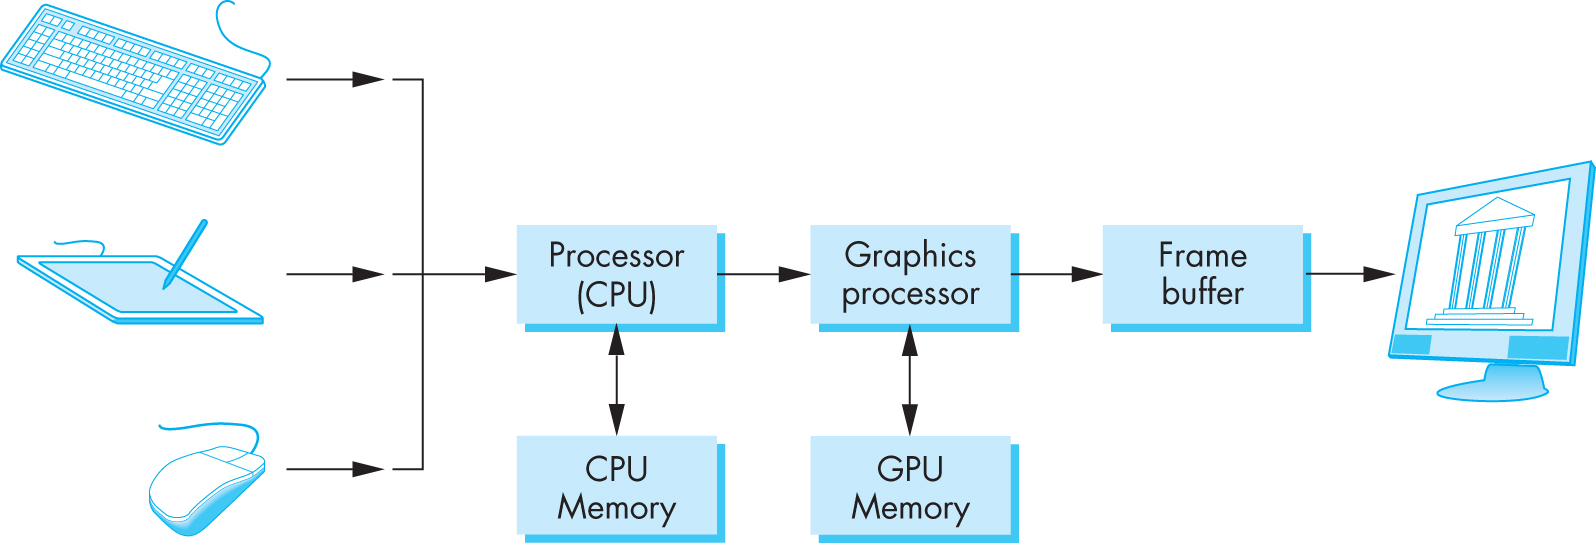
\includegraphics[width=\columnwidth]{graphics-system.jpg}
\end{figure}

프레임버퍼는 그래픽스 시스템의 핵심 요소로 각 픽셀의 정보(색상, 명암 등)에 대한 정보를 디스플레이 크기만큼 저장하고 있음. 즉, 화면 정보를 변경하는 것은 프레임버퍼를 변경하는 것. 커서를 움직이면 프레임버퍼 내용이 바뀐다.

프레임버퍼에 내용을 그릴 때마다 즉시 화면을 갱신하면 깜박임이 생김. 화면을 그릴 때 이전 프레임을 지우는 과정이 보이기 때문. 그래서 별도의 버퍼(back buffer)에 화면을 다 그려놓고 front buffer와 교체(swap)한다. 즉, back buffer는 쓰기 전용, front buffer는 읽기 전용으로 사용. 이를 double buffering이라고 함.

오늘날 대부분의 그래픽스 시스템은 래스터 베이스. 이미지가 프레임버퍼에 있는 픽셀의 배열로 만들어짐. 해상도는 프레임 버퍼에 있는 픽셀의 개수에, 선명도는 각 픽셀이 얼마나 많은 색을 표현할 수 있는지(사용하는 비트 수)에 따른다. 1비트는 2가지 색, 8비트는 256가지 색(RGB 당 8비트). 요즘엔 10비트, 12비트도 쓰인다. 그래픽스 파이프라인은 3차원 개체를 2차원 래스터 이미지로 표현하기 위한 일련의 처리 과정.

\begin{figure}[h]
  \centering
  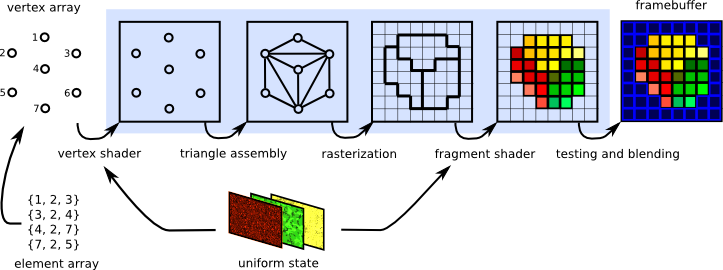
\includegraphics[width=\columnwidth]{graphics-pipeline.png}
\end{figure}

\begin{enumerate}
  \item vertex processor: 정점의 위치와 카메라의 위치, 원근법 등을 조정한다. 3차원 상의 점을 2차원 상의 점으로 표현한다.
  \item clipper and primitive assembler: 카메라에 보이지 않는 물체를 잘라내고(clipping) 각 정점을 이어 객체를 구성(primitive assembly)한다.
  \item rasterizer: 객체가 픽셀의 배열(raster)로 이뤄진 화면에서 어떤 픽셀에 해당하는지 계산하여 프래그먼트 집합을 구성한다.
  \item fragment processor: 프래그먼트에 색을 표현한다. 음영이나 깊이감이 반영된다.
\end{enumerate}

대부분 하드웨어에 구현되어 있기 때문에 우리는 vertex processor(vertex shader)와 gragment processor(fragment shader)에 개입한다.

\section{Geometry}

\begin{figure}[h]
  \centering
  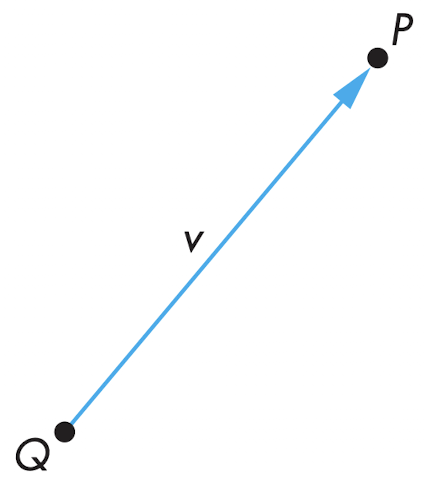
\includegraphics[width=3cm]{point-point-to-vector.png}
\end{figure}

기하학의 기본적인 3 요소는 스칼라, 벡터, 점.

\begin{itemize}
  \item 스칼라: 크기
  \item 벡터: 방향과 길이
    \begin{itemize}
      \item 모든 벡터는 인버스를 갖는다: $\bold{v}$, $-\bold{v}$
      \item 모든 벡터에는 스칼라를 곱할 수 있다: $\alpha \bold{v}$ ($\alpha$가 0이라면 영벡터)
      \item 영벡터: 길이 0, 방향이 정해지지 않은 벡터.
      \item 어떤 두 벡터의 합은 벡터다: $\bold{u} + \bold{w} = \bold{v}$
      \item 벡터 공간에서 벡터에는 위치가 없기 때문에 방향과 길이가 같다면 어디에 있든 모두 같은 벡터.
    \end{itemize}
  \item 점: 공간 위의 어떤 위치
    \begin{itemize}
      \item 벡터는 두 점의 위치 차를 표현한 것.
      \item 따라서 점-점 뺄셈의 결과는 벡터: $\bold{v} = P - Q$, $P = Q + \bold{v}$
    \end{itemize}
\end{itemize}

\subsection{Affine Spaces}

벡터 공간을 확장해 점과 벡터가 관계를 맺는 공간. 원점이 어디인지 모르는 벡터 공간이기도 하다. 벡터 공간과 달리 아핀 공간에는 위치를 특정하는 점에 대한 개념이 있음. 따라서 아래와 같은 연산이 가능하다.

\begin{itemize}
  \item 벡터-벡터 덧셈 $\rightarrow$ 벡터
  \item 벡터-스칼라 곱셈 $\rightarrow$ 벡터
  \item 점-점 뺄셈 $\rightarrow$ 벡터
  \item 점-벡터 덧셈 $\rightarrow$ 점
  \item 점-점 덧셈 $\rightarrow$ ???
\end{itemize}

모든 점은 $P(\alpha) = P_0 + \alpha d$와 같이 표현 가능하다. 이때 $P_0$는 임의의 점, $d$는 임의의 벡터, $\alpha$는 스칼라다. $\alpha$가 주어지면 직선을 얻을 수 있으며, 여기서 $\alpha$는 직선과 관계없이 '매개'하는 역할만 하므로 이러한 표현은 parametric form. 직선을 표현하는 경우:

\begin{itemize}
  \item explicit: $y = mx + h$, $x$를 알면 $y$를 구할 수 있음. y축과 평행한 직선은 표현 불가.
  \item implicit: $ax + by + c = 0$, $x$, $y$를 알면 직선 위의 점인지 알 수 있음.
  \item parametric: $x(\alpha) = \alpha x_0 + (1 - \alpha)x_1$, $y(\alpha) = \alpha y_0 + (1 - \alpha)y_1$
\end{itemize}

원의 방정식의 경우 implicit form으로 $x^2 - y^2 = 1$인데, parametric으로는 $x = \cos{\theta}, y = \sin{\theta}$임.

\subsection{Affine Sums}

원래 점-점 덧셈과 점-스칼라 곱셈은 불가능하지만 아핀 합으로는 할 수 있다.

\begin{itemize}
  \item 각 점들 앞의 계수($\alpha$) 합이 1일 때 점-점 덧셈이 허용.
  \item $n$개의 점의 덧셈에서 계수의 합이 1이 되는 경우를 아핀 합이라고 한다.
\end{itemize}

어떤 점 $Q$, 벡터 $\bold{v}$, 스칼라 $\alpha$가 있을 때,

\begin{figure}[h]
  \centering
  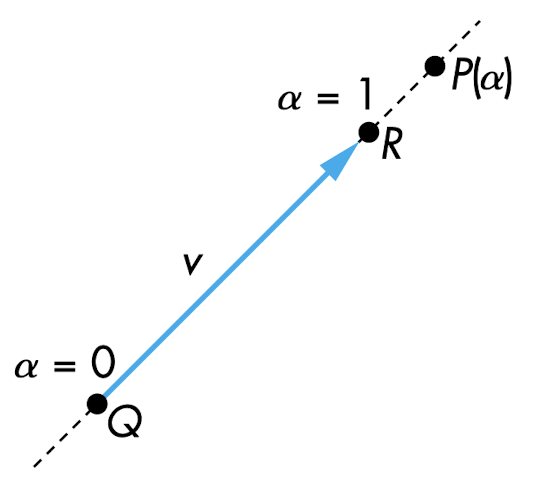
\includegraphics[width=5cm]{point-q-to-r.png}
\end{figure}

점 $Q$에서 $\bold{v}$ 방향의 직선 위에 있는 모든 점을 아래와 같은 parametric form으로 표현할 수 있다.
$$P = Q + \alpha \bold{v}$$
이때 다음을 만족하는 점 $R$을 항상 찾을 수 있다.
$$
\begin{aligned}
  \bold{v} &= R - Q \\
  \therefore P &= Q + \alpha (R - Q) = \alpha R + (1 - \alpha) Q
\end{aligned}
$$
이는 점-점 덧셈으로 볼 수도 있다.
$$P = \alpha_1 R + \alpha_2 Q \quad \text{where} \quad \alpha_1 + \alpha_2 = 1$$
따라서 아핀 공간에서는 점-점 덧셈이 가능하다.

\subsection{Convexity}

convex는 개체 내 임의의 두 점을 선택했을 때 두 점을 이은 선이 해당 개체 안에 포함되는 것. $n$개의 점 $P_1, P_2, \cdots, P_n$으로 정의되는 개체에 대한 아핀 합은 아래와 같다.
$$P = \alpha_1 P_1 + \alpha_2 P_2 + \cdots + \alpha_n P_n$$
다음 조건을 만족할 때 위의 식이 의미를 가짐을 귀납적으로 보일 수 있다.
$${\alpha}_1 + {\alpha}_2 + \cdots + {\alpha}_n = 1$$
이를 만족하는 점 $P$들은 모두 개체 안에 포함된다.

convex hull은 점 $P_1, P_2, \cdots P_n$들을 모두 포함하는 최소의 convex 개체. $\alpha_i >= 0$이면 $P_1, P_2, \cdots P_n$의 convex hull이 된다.

삼각형은 convex하기 때문에 내부에 있는 어떤 점을 아핀 합으로 표현할 수 있다
$$
\begin{aligned}
  P(\alpha_1, \alpha_2, \alpha_3) = \alpha_1P + \alpha_2Q + \alpha_3R \\
  \text{where} \quad \alpha_1 + \alpha_2 + \alpha_3 = 1, \quad \alpha_i >= 0
\end{aligned}
$$
후술할 무게 중심과 관련있다.

\subsection{Dot and Cross Products}

$|\bold{v}|$는 벡터 $\bold{v}$의 길이.
\begin{itemize}
  \item $|\bold{v}| = \sqrt{{\bold{v}_x}^2 + {\bold{v}_y}^2 + {\bold{v}_z}^2}$
  \item $\bold{v} \cdot \bold{v} = |\bold{v}|^2$
\end{itemize}

\subsubsection{Dot(inner) Product}

$$\bold{u} \cdot \bold{v}$$

두 벡터 사이의 스칼라(두 벡터의 사이각 등)를 구할 때, 폴리곤의 안팎을 구별할 때 사용. $\bold{u} \cdot \bold{v} = 0$이라면 두 벡터는 수직이다.

아래와 같은 두 벡터 사이각의 코사인은

\begin{figure}[h]
  \centering
  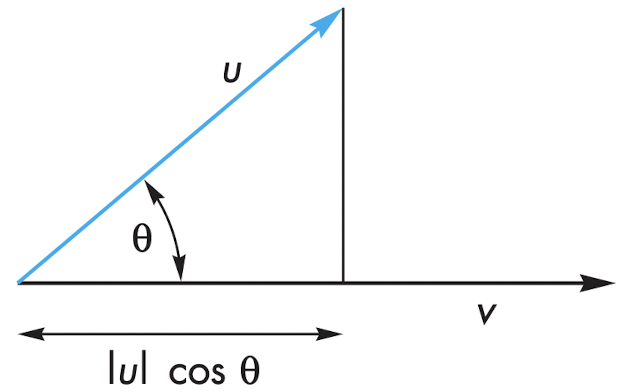
\includegraphics[width=5cm]{two-vectors-cos.png}
\end{figure}

$$
\begin{aligned}
  \bold{u} \cdot \bold{v} &= |\bold{u}| |\bold{v}| \cos{\theta} \\
  \therefore \cos{\theta} &= {{\bold{u} \cdot \bold{v}} \over |\bold{u}| |\bold{v}|}
\end{aligned}
$$
코사인 값은 두 벡터가 가까워지면 1, 멀어지면 0(수직)이 된다. 피사체가 카메라 앞에 있는지, 뒤에 있는지 계산: 카메라의 정면으로 향하는 벡터 $\bold{u}$와 피사체로 향하는 벡터 $\bold{v}$가 있을 때 $\bold{u} \cdot \bold{v} \over |\bold{u}| |\bold{v}|$가 0보다 크면 앞, 0보다 작으면 뒤에 있는 것. ($\because$ 앞뒤는 180도를 기준으로 판단, -90도에서 90도 사이에 피사체가 있다면 앞에 있는 것이므로.)

\begin{framed}
  \noindent \textbf{예시}: $\bold{u} = (1, 2, 3), \bold{v} = (4, -5, 6)$
  $$
  \begin{aligned}
    \bold{u} \cdot \bold{v} &= \bold{u}_1 \bold{v}_1 + \bold{u}_2 \bold{v}_2 + \bold{u}_3 \bold{v}_3 \\
    &= 1(4) + 2(-5) + 3(6) \\
    &= 12
  \end{aligned}
  $$
\end{framed}

\begin{figure}[h]
  \centering
  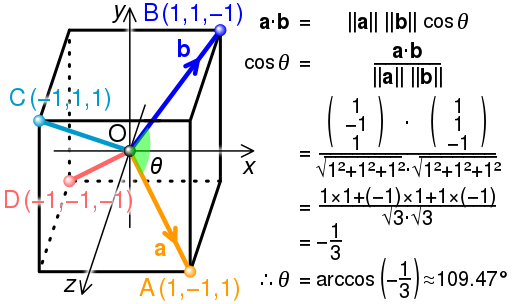
\includegraphics[width=\columnwidth]{tetrahedral-angle-calculation.png}
\end{figure}

\subsubsection{Cross(outer) Product}

$$\bold{u} \times \bold{v}$$

3차원에서 두 벡터와 수직인 벡터를 구할 때, 한 평면의 normal vector를 구할 때 사용.

\begin{figure}[h]
  \centering
  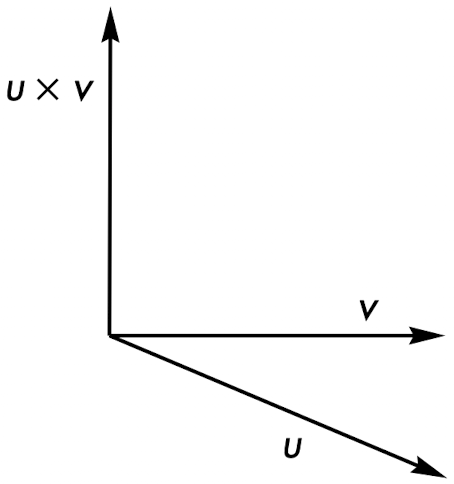
\includegraphics[width=3cm]{cross-product-normal-vector.png}
\end{figure}

$$
\begin{aligned}
  \bold{u} \times \bold{v} &= |\bold{u}| |\bold{v}| \sin{\theta} \\
  \therefore \sin{\theta} &= {\bold{u} \times \bold{v} \over |\bold{u}| |\bold{v}|}
\end{aligned}
$$
$\bold{v} = (v_1, v_2, v_3), \bold{w} = (w_1, w_2, w_3)$인 경우 $\bold{v} \times \bold{w}$:
$$
\begin{aligned}
  \bold{v} \times \bold{w} &=
  \begin{bmatrix}
    \bold{i} & \bold{j} & \bold{k} \\
    v_1 & v_2 & v_3 \\
    w_1 & w_2 & w_3
  \end{bmatrix} \\
  &= (v_2 w_3 - v_3 w_2)\bold{i} + (v_3 w_1 - v_1 w_3)\bold{j} \\
  &\quad + (v_1 w_2 - v_2 w_1)\bold{k}
\end{aligned}
$$
사실 $\bold{j}$의 스칼라 부분 연산은 $(v_3 w_1 - v_1 w_3)\bold{j}$로 순서가 반대이지만, 시각적으로 연산 순서를 기억하기 쉽도록 $\bold{j}$의 부호를 음의 부호로 바꿔서 표현할 수 있다.
$$
(v_2 w_3 - v_3 w_2)\bold{i} \underline{- (v_1 w_3 - v_3 w_1)\bold{j}} + (v_1 w_2 - v_2 w_1)\bold{k}
$$

\begin{framed}
  \noindent \textbf{예시}: $\bold{v} = (3, -3, 1), \bold{w} = (4, 9, 2)$
  $$
  \begin{aligned}
    \bold{v} \times \bold{w} &=
    \begin{bmatrix}
      \bold{i} & \bold{j} & \bold{k} \\
      3 & -3 & 1 \\
      4 & 9 & 2
    \end{bmatrix} \\
    &= [-3(2) - 1(9)]\bold{i} - [3(2) - 1(4)]\bold{j} \\
    &\quad + [3(9) - -3(4)]\bold{k} \\
    &= -15\bold{i} - 2\bold{j} + 39\bold{k}
  \end{aligned}
  $$
\end{framed}

\begin{framed}
  \noindent \textbf{예시}: 점 $P(0, 0, 0), Q(2, 4, 6), R(-1, 2, 7)$로 이뤄진 평면의 법선 벡터는 벡터 $Q - P$와 벡터 $R - P$에 공통으로 수직인 벡터.
  $$
  \begin{aligned}
    \bold{v} &= Q - P = (2, 4, 6) - (0, 0, 0) = (2, 4, 6) \\
    \bold{w} &= R - P = (-1, 2, 7) - (0, 0, 0) = (-1, 2, 7) \\
  \end{aligned}
  $$
  $$
  \begin{aligned}
    \bold{v} \times \bold{w} &=
    \begin{bmatrix}
      \bold{i} & \bold{j} & \bold{k} \\
      2 & 4 & 6 \\
      -1 & 2 & 7
    \end{bmatrix} \\
    &= [4(7) - 6(2)]\bold{i} - [2(7) - 6(-1)]\bold{j} \\
    &\quad + [2(2) - 4(-1)]\bold{k} \\
    &= 16\bold{i} - 20\bold{j} + 8\bold{k} \\
    &= (16, -20, 8)
  \end{aligned}
  $$
\end{framed}

\subsection{Planes}

평면은 하나의 점과 두 개의 벡터, 또는 세 개의 점으로 정의할 수 있다. 하나의 점, 두 개의 벡터로 정의하는 경우
$$P(\alpha, \beta) = R + \alpha \bold{u} + \beta \bold{v}$$
세 개의 점으로 정의하는 경우
$$P(\alpha, \beta) = R + \alpha (Q - R) + \beta (P - Q)$$

아래와 같이 아핀 공간의 점 $P, Q, R$로 정의된 삼각형이 있을 때,

\begin{figure}[h]
  \centering
  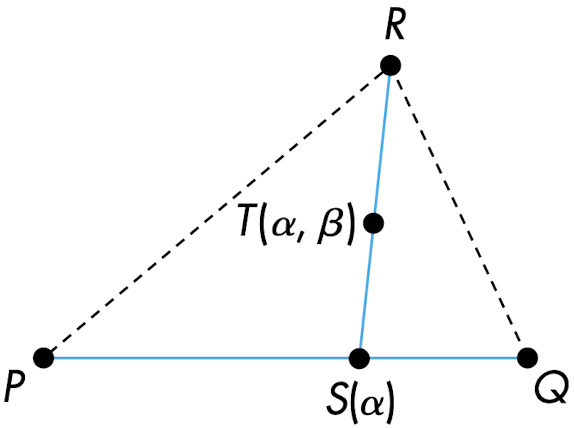
\includegraphics[width=5cm]{affine-space-triangle.png}
\end{figure}

점 $P, Q$를 잇는 선 위에 있는 임의의 점 $S$는
$$S(\alpha) = \alpha P + (1 - \alpha)Q, \quad 0 \leq \alpha \leq 1$$
점 $S, R$을 잇는 선 위에 있는 임의의 점 $T$는
$$T(\beta) = \beta S + (1 - \beta)R, \quad 0 \leq \beta \leq 1$$
점 $S, T$는 $\alpha, \beta$로 결정되며, 면은 $P, Q, R$로 결정되므로 아래와 같은 삼각형 평면의 방정식을 얻을 수 있다.
$$
\begin{aligned}
  T(\alpha, \beta) &= \beta[\alpha P + (1 - \alpha)Q] + (1 - \beta)R \\
  &= P + \beta(1 - \alpha)(Q - P) + (1 - \beta)(R - P)
\end{aligned}
$$
$Q - P$와 $R - P$는 임의의 벡터이므로, 이를 각각 $\bold{u}, \bold{v}$로 바꾸면 하나의 점과 두 개의 벡터로 평면을 표현하는 셈이 된다.
$$
\begin{aligned}
  T(\alpha, \beta) &= P_0 + \alpha \bold{u} + \beta \bold{v} \\
  &= \beta \alpha P + \beta(1 - \alpha)Q + (1 - \beta)R \\
  T(\alpha, \beta^\prime, \gamma) &= \alpha^\prime P + \beta^\prime Q + \gamma^\prime R \\
  \text{where} \quad &\alpha^\prime + \beta^\prime + \gamma^\prime = 1
\end{aligned}
$$
이때 $(\alpha^\prime, \beta^\prime, \gamma^\prime)$을 무게중심 좌표(barycentric coordinate)라고 한다. 삼각형 내에 있는 점 T에 대한 barycentric coordinate 표현은
$$
\begin{aligned}
  T &= \beta \bold{u} + \gamma \bold{v} + P \\
  &= \beta(Q - P) + \gamma(R - P) + P \\
  &= \underbrace{(1 - \beta - \gamma)}_{\alpha}P + \beta Q + \gamma R
\end{aligned}
$$
이때 무게중심 좌표는 $(\alpha, \beta, \gamma)$. 앞서 본 $T(\alpha, \beta) = P_0 + \alpha \bold{u} + \beta \bold{v}$로부터 $\bold{u} \times \bold{v}$(평면에 직교하는 normal vector)를 구하면 평면을 표현하는 또 다른 방정식을 얻을 수 있다.
$$\bold{u} \times \bold{v} \cdot (P - P_0) = 0$$

\section{3D Object Modeling}

\subsection{Polygonal Representation}

boundary representations은 외부에 보이는 표면만 모델링하는 방식. 점을 이어서 망(mesh)를 만든다. 직관적이고 단순한 방법으로 대부분 이 방식으로 모델링한다. 사용자 친화적이지 않고 기계 친화적이라는 단점이 있음.

보통 폴리곤은 삼각형으로 모델링한다. 삼각형은 완전히 평면적임을 보장할 수 있고, cross product로 평면이 어느 쪽을 바라보고 있는지 쉽게 구할 수 있기 때문. 삼각형을 사용하면 임의의 점 3개로 유니크한 평면을 만들 수 있다. 단, 점 3개가 같은 직선 상에 있다면, 또는 두 벡터가 같은 방향이라면 유니크한 평면이 불가능하다.

만약 점 4개를 선택한다면 유니크한 평면을 만들지 못하고 사각형이 아니라 삼각뿔을 만들게 될 수 있다.

폴리곤을 어떻게 저장할까?

\begin{itemize}
  \item Face Set (STL): 삼각형을 구성하는 3개의 점 좌표를 모두 저장하는 방식.
    \begin{itemize}
      \item 같은 점에 대한 중복 데이터를 저장하게 되는 문제.
      \item 한 점의 위치를 변경하면 그 점을 참조하는 삼각형 전체의 위치가 바뀜.
    \end{itemize}
  \item Shared Vertex (OBJ, OFF): 점과 삼각형 정보를 따로 저장하는 방식.
    \begin{itemize}
      \item vertices 테이블에는 점의 x, y, z 좌표, triangles 테이블에는 하나의 삼각형을 구성하는 3개의 점을 참조.
      \item triangles:vertices를 1:N 데이터베이스로 구성하는 형태.
    \end{itemize}
\end{itemize}

\subsection{Other Representations}

\begin{itemize}
  \item Sweep: 평면을 회전시켜 입체 도형을 표현. 쉽게 안팎을 구별할 수 있음.
  \item Fractal: 프랙탈로 표현. 멀리서는 물체가 한 덩어리로 보이다가 가까워질수록 정교하게 보임.
  \item Constructive Solid Geometry: 집합 연산(union, intersection, difference)를 이용해 도형을 표현. 겉부분이 아니라 보이지 않는 내부까지 구현해야 할 때 사용.
  \item Quadtree: 트리로 표현. 트리가 깊어질수록 정교한 표현. 중간 정도에서는 개략적인 모양을 얻을 수 있음.
  \item Voxel: 2차원 평면을 쌓아 부피를 만들어 표현.
  \item Implicit Surface: $f(\bold{p}) = Q$를 만족하는 점의 집합으로 표현.
\end{itemize}

\subsection{Vertex Array and Buffer}

매 프레임마다 RAM으로부터 CPU를 거쳐 GPU로 데이터를 불러오면 CPU와 CPU-GPU 사이 버스에 오버헤드가 커짐. 특히 프레임 사이 변경이 크게 없다면 불필요한 데이터를 계속 불러오는 것. 그래서 프로그램을 로드할 때 GPU에 데이터를 보내두고 매 프레임 데이터는 GPU가 처리.

\begin{figure}[h]
  \centering
  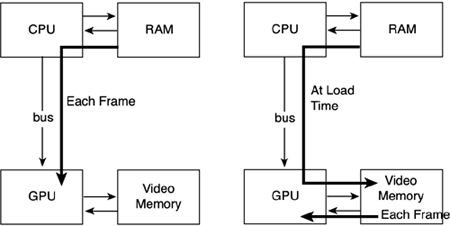
\includegraphics[width=\columnwidth]{ram-cpu-gpu-video-memory.png}
\end{figure}

\begin{itemize}
  \item Vertex Buffer Object(VBO): vertex data를 받아 GPU 메모리에 전달하기 위한 버퍼.
  \item Vertex Array Object(VAO): vertex buffer와 연결된 배열. vertex attributes를 담고 있으며, vertex shader가 이 attributes를 참조해 렌더링을 한다.
\end{itemize}

아래와 같은 과정을 거친다.

\begin{enumerate}
  \item 새로운 VBO 생성
  \item 버퍼 바인딩
  \item 비디오 메모리 공간 할당 및 vertex 데이터를 버퍼 객체에 복사
  \item 새로운 VAO 생성
  \item 배열 바인딩
  \item vertex attribute 배열 정의 및 VBO와 VAO 연결.
\end{enumerate}

\section{2D Geometric Transformation}

2D 평면을 변형(이동: translation, 회전: rotation, 신축: scaling)한다. 어떤 점 $\bold{p}$를 2D에서는 $\bold{p} = (x, y)$, 3D에서는 $\bold{p} = (x, y, z)$로 표현한다. 이를 컬럼 벡터로 표현할 수도 있다.
$$
\bold{p} =
\begin{bmatrix}
  x \\
  y
\end{bmatrix}
\quad \text{or} \quad
\bold{p} =
\begin{bmatrix}
  x \\
  y \\
  z
\end{bmatrix}
$$
2D 변형을 행렬 $M$으로 표현하여 컬럼 벡터 $\bold{p}$에 적용하면: $\bold{p}^\prime = M\bold{p}$
$$
\begin{bmatrix}
  x^\prime \\
  y^\prime
\end{bmatrix}
{=}
\begin{bmatrix}
  a & b \\
  c & d
\end{bmatrix}
\begin{bmatrix}
  x \\
  y
\end{bmatrix}
{=}
\begin{bmatrix}
  ax + by \\
  cx + dy
\end{bmatrix}
$$

\subsection{Translation}

점 $\bold{p}$를 $\bold{t}$만큼 이동시켜 점 $\bold{p}^\prime$으로 변형한다: $\bold{p}^\prime = \bold{p} + \bold{t}$
$$
\bold{p}^\prime =
\begin{bmatrix}
  x^\prime \\
  y^\prime
\end{bmatrix}
\quad
\bold{p} =
\begin{bmatrix}
  x \\
  y
\end{bmatrix}
\quad
\bold{t} =
\begin{bmatrix}
  t_x \\
  t_y
\end{bmatrix}
$$
$$
\bold{p}^\prime =
\begin{bmatrix}
  x \\
  y
\end{bmatrix}
{+}
\begin{bmatrix}
  t_x \\
  t_y
\end{bmatrix}
=
\begin{bmatrix}
  x + t_x \\
  y + t_y
\end{bmatrix}
$$

\subsection{Rotation}

점 $\bold{p}$를 $\theta$만큼 회전시켜 점 $\bold{p}^\prime$으로 변형: $\bold{p}^\prime = R(\theta)\bold{p}$
$$
\bold{p}^\prime =
\begin{bmatrix}
  x^\prime \\
  y^\prime
\end{bmatrix}
\quad
\bold{p} =
\begin{bmatrix}
  x \\
  y
\end{bmatrix}
\quad
R(\theta) =
\begin{bmatrix}
  \cos{\theta} & -\sin{\theta} \\
  \sin{\theta} & \cos{\theta}
\end{bmatrix}
$$
$$
\bold{p}^\prime =
\begin{bmatrix}
  \cos{\theta} & -\sin{\theta} \\
  \sin{\theta} & \cos{\theta}
\end{bmatrix}
\begin{bmatrix}
  x \\
  y
\end{bmatrix}
=
\begin{bmatrix}
  x\cos{\theta} - y\sin{\theta} \\
  x\sin{\theta} + y\cos{\theta}
\end{bmatrix}
$$

\subsection{Scaling}

점 $\bold{p}$를 x축으로 $s_x$배, y축으로 $s_y$배만큼 신축해 점 $\bold{p}^\prime$으로 변형한다: $\bold{p}^\prime = S(s_x, s_y)\bold{p}$
$$
\bold{p}^\prime =
\begin{bmatrix}
  x^\prime \\
  y^\prime
\end{bmatrix}
\quad
\bold{p} =
\begin{bmatrix}
  x \\
  y
\end{bmatrix}
\quad
S(s_x, s_y) =
\begin{bmatrix}
  s_x & 0 \\
  0 & s_y
\end{bmatrix}
$$
$$
\bold{p}^\prime =
\begin{bmatrix}
  s_x & 0 \\
  0 & s_y
\end{bmatrix}
\begin{bmatrix}
  x \\
  y
\end{bmatrix}
=
\begin{bmatrix}
  s_x x \\
  s_y y
\end{bmatrix}
$$

\subsection{Homogeneous Coordinates}

앞서 translation은 scaling, rotation과 다르게 행렬 합으로 표현했다. 그런데 homogeneous coordination을 사용하면 모든 변형을 행렬 곱으로 표현할 수 있다.

2D 좌표계 $(x, y)$를 확장해 세 개의 요소로 표현할 수 있음: $(x_h, y_h, h)$. 이를 다시 cartesian coordinates로 표현하면: $x = {x_h \over h}$, $y = {y_h \over h}$ 일반적으로 $h$는 1로 둔다. $(x_h, y_h, 0)$이면 점의 좌표가 무한하다는 의미. $(2, 1, 1) = (4, 2, 2) = (6, 3, 3)$. $(0, 0, 0)$은 불가능.

\subsubsection{Translation}

$$\bold{p}^\prime = T(t_x, t_y)\bold{p}$$
$$
\begin{bmatrix}
  x^\prime \\
  y^\prime \\
  1
\end{bmatrix}
{=}
\begin{bmatrix}
  1 & 0 & t_x \\
  0 & 1 & t_y \\
  0 & 0 & 1
\end{bmatrix}
\begin{bmatrix}
  x \\
  y \\
  1
\end{bmatrix}
{=}
\begin{bmatrix}
  x + t_x \\
  y + t_y \\
  1
\end{bmatrix}
$$
$$T^{-1}(t_x, t_y) = T(-t_x, -t_y)$$
$$T(t_{x2}, t_{y2}) \cdot T(t_{x1}, t_{y1}) = T(t_{x1} + t_{x2}, t_{y1} + t_{y2})$$

\subsubsection{Rotation}

$$\bold{p}^\prime = R(\theta)\bold{p}$$
$$
\begin{bmatrix}
  x^\prime \\
  y^\prime \\
  1
\end{bmatrix}
{=}
\begin{bmatrix}
  \cos{\theta} & -\sin{\theta} & 0 \\
  \sin{\theta} & \cos{\theta} & 0 \\
  0 & 0 & 1
\end{bmatrix}
\begin{bmatrix}
  x \\
  y \\
  1
\end{bmatrix}
$$
$$R^{-1}(\theta) = R(-\theta)$$
$$R(\theta_2) \cdot R(\theta_1) = R(\theta_1 + \theta_2)$$

\subsubsection{Scaling}

$$\bold{p}^\prime = S(s_x, s_y)\bold{p}$$
$$
\begin{bmatrix}
  x^\prime \\
  y^\prime \\
  1
\end{bmatrix}
{=}
\begin{bmatrix}
  s_x & 0 & 0 \\
  0 & s_y & 0 \\
  0 & 0 & 1
\end{bmatrix}
\begin{bmatrix}
  x \\
  y \\
  1
\end{bmatrix}
$$
$$S^{-1}(s_x, s_y) = S({1 \over s_x}, {1 \over s_y})$$
$$S(s_{x2}, s_{y2}) \cdot S(s_{x1}, s_{y1}) = S(s_{x1} \cdot s_{x2}, s_{y1} \cdot s_{y2})$$

\subsection{Pivot-Point Transformations}

원점에서 변형하는 것과 달리 특정 점을 기준으로 회전, 신축 변환하려면 절차가 더 필요하다. 일단 개체를 원점으로 옮겨서 변환하고, 다시 원래 자리로 돌려 놓아야 함. 주의: $\bold{v}$에 $A, B, C$ 순서로 적용한다면 $C(B(A\bold{v})) = CBA(\bold{v})$이다.

\subsubsection{Rotation}

\begin{figure}[h]
  \centering
  \includegraphics[width=\columnwidth]{pivot-point-Transformations-rotation.png}
\end{figure}

\begin{enumerate}[(a)]
  \item 개체의 원위치는 $(x_r, y_r)$.
  \item 개체를 좌표계의 원점으로 이동(translation).
  \item 개체를 회전(rotation).
  \item 개체를 다시 원위치로 이동(translation).
\end{enumerate}
$$
\begin{aligned}
  R&(x_r, y_r, \theta) \\
  &= \overbrace{T(x_r, y_r)}^{(d)} \cdot \overbrace{R(\theta)}^{(c)} \cdot \overbrace{T(-x_r, -y_r)}^{(b)} \\
  &=
  \begin{bmatrix}
    1 & 0 & x_r \\
    0 & 1 & y_r \\
    0 & 0 & 1
  \end{bmatrix}
  \begin{bmatrix}
    \cos{\theta} & -\sin{\theta} & 0 \\
    \sin{\theta} & \cos{\theta} & 0 \\
    0 & 0 & 1
  \end{bmatrix}
  \begin{bmatrix}
    1 & 0 & -x_r \\
    0 & 1 & -y_r \\
    0 & 0 & 1
  \end{bmatrix} \\
  &=
  \begin{bmatrix}
    \cos{\theta} & -\sin{\theta} & x_r \\
    \sin{\theta} & \cos{\theta} & y_r \\
    0 & 0 & 1
  \end{bmatrix}
  \begin{bmatrix}
    1 & 0 & -x_r \\
    0 & 1 & -y_r \\
    0 & 0 & 1
  \end{bmatrix} \\
  &=
  \begin{bmatrix}
    \cos{\theta} & -\sin{\theta} & -x_r\cos{\theta} + y_r\sin{\theta} + x_r \\
    \sin{\theta} & \cos{\theta} & -x_r\sin{\theta} - y_r\cos{\theta} + y_r \\
    0 & 0 & 1
  \end{bmatrix}
\end{aligned}
$$
\begin{framed}
  \noindent \textbf{예시}: 점 $A(4, 6), B(2, 2), C(6, 2)$으로 정의된 삼각형 $T$를 고정점 $(3, 3)$ 기준 반시계 방향으로 90도 회전시켰을 때 $T^\prime$이라고 하면
  $$
  \begin{aligned}
    &R(3, 3, {\pi \over 2}) = T(3, 3) \cdot R({\pi \over 2}) \cdot T(-3, -3) \\
    &=
    \begin{bmatrix}
      1 & 0 & 3 \\
      0 & 1 & 3 \\
      0 & 0 & 1
    \end{bmatrix}
    \begin{bmatrix}
      \cos{\pi \over 2} & -\sin{\pi \over 2} & 0 \\
      \sin{\pi \over 2} & \cos{\pi \over 2} & 0 \\
      0 & 0 & 1
    \end{bmatrix}
    \begin{bmatrix}
      1 & 0 & -3 \\
      0 & 1 & -3 \\
      0 & 0 & 1
    \end{bmatrix} \\
    &=
    \begin{bmatrix}
      \cos{\pi \over 2} & -\sin{\pi \over 2} & 3 \\
      \sin{\pi \over 2} & \cos{\pi \over 2} & 3 \\
      0 & 0 & 1
    \end{bmatrix}
    \begin{bmatrix}
      1 & 0 & -3 \\
      0 & 1 & -3 \\
      0 & 0 & 1
    \end{bmatrix} \\
    &=
    \begin{bmatrix}
      \cos{\pi \over 2} & -\sin{\pi \over 2} & -3 \cos{\pi \over 2} + 3 \sin{\pi \over 2} + 3 \\
      \sin{\pi \over 2} & \cos{\pi \over 2} & -3 \sin{\pi \over 2} - 3 \cos{\pi \over 2} + 3 \\
      0 & 0 & 1
    \end{bmatrix} \\
    &=
    \begin{bmatrix}
      0 & -1 & 6 \\
      1 & 0 & 0 \\
      0 & 0 & 1
    \end{bmatrix} \\
  \end{aligned}
  $$
  $$
  \begin{aligned}
    \therefore T^\prime &= R(3, 3, {\pi \over 2}) \cdot T \\
    &=
    \begin{bmatrix}
      0 & -1 & 6 \\
      1 & 0 & 0 \\
      0 & 0 & 1
    \end{bmatrix}
    \begin{bmatrix}
      4 & 2 & 6 \\
      6 & 2 & 2 \\
      1 & 1 & 1
    \end{bmatrix} \\
    &=
    \begin{bmatrix}
      0 & 4 & 4 \\
      4 & 2 & 6 \\
      1 & 1 & 1
    \end{bmatrix}
    \quad
    \begin{aligned}
      A^\prime = (0, 4) \\
      B^\prime = (4, 2) \\
      C^\prime = (4, 6)
    \end{aligned}
  \end{aligned}
  $$
\end{framed}

\subsubsection{Scaling}

\begin{figure}[h]
  \centering
  \includegraphics[width=\columnwidth]{pivot-point-Transformations-scaling.png}
\end{figure}

\begin{enumerate}[(a)]
  \item 개체의 원위치는 $(x_f, y_f)$.
  \item 개체를 좌표계의 원점으로 이동(translation).
  \item 개체를 확대/축소(scaling).
  \item 개체를 다시 원위치로 이동(translation).
\end{enumerate}
$$
\begin{aligned}
  S&(x_f, y_f, s_x, s_y) \\
  &= \overbrace{T(x_f, y_f)}^{(d)} \cdot \overbrace{S(s_x, s_y)}^{(c)} \cdot \overbrace{T(-x_f, -y_f)}^{(b)} \\
  &=
  \begin{bmatrix}
    1 & 0 & x_f \\
    0 & 1 & y_f \\
    0 & 0 & 1
  \end{bmatrix}
  \begin{bmatrix}
    s_x & 0 & 0  \\
    0 & s_y & 0 \\
    0 & 0 & 1
  \end{bmatrix}
  \begin{bmatrix}
    1 & 0 & -x_f \\
    0 & 1 & -y_f \\
    0 & 0 & 1
  \end{bmatrix} \\
  &=
  \begin{bmatrix}
    s_x & 0 & x_f \\
    0 & s_y & y_f \\
    0 & 0 & 1
  \end{bmatrix}
  \begin{bmatrix}
    1 & 0 & -x_f \\
    0 & 1 & -y_f \\
    0 & 0 & 1
  \end{bmatrix} \\
  &=
  \begin{bmatrix}
    s_x & 0 & -s_x x_f + x_f \\
    0 & s_y & -s_y y_f + y_f \\
    0 & 0 & 1
  \end{bmatrix}
\end{aligned}
$$

\subsection{Other Transformations}

\subsubsection{Reflection}

x축을 기준으로 반사:
$
\begin{bmatrix}
  1 & 0 & 0 \\
  0 & -1 & 0 \\
  0 & 0 & 1
\end{bmatrix}
$
\\
y축을 기준으로 반사:
$
\begin{bmatrix}
  -1 & 0 & 0 \\
  0 & 1 & 0 \\
  0 & 0 & 1
\end{bmatrix}
$
\\
원점을 기준으로 반사:
$
\begin{bmatrix}
  -1 & 0 & 0 \\
  0 & -1 & 0 \\
  0 & 0 & 1
\end{bmatrix}
$
\\
직선 $y = x$를 기준으로 반사:
$
\begin{bmatrix}
  0 & 1 & 0 \\
  1 & 0 & 0 \\
  0 & 0 & 1
\end{bmatrix}
$

\subsubsection{Shear}

직선 $y = y_{ref}$에 x축 방향:
$
\begin{bmatrix}
  1 & sh_x & -sh_x \cdot y_{ref} \\
  0 & 1 & 0 \\
  0 & 0 & 1
\end{bmatrix}
$
\\
직선 $x = x_{ref}$에 y축 방향:
$
\begin{bmatrix}
  1 & 0 & 0 \\
  sh_y & 1 & -sh_y \cdot x_{ref} \\
  0 & 0 & 1
\end{bmatrix}
$

\subsection{Change of Coordinate Systems}

새로운 좌표축을 그려서 기존 개체를 다루고 싶을 때는 좌표축의 변형 과정을 역으로 하면 된다. 만약 축을 이동, 회전했다면 아래와 같이 한다.
$$
T(-x_0, -y_0) =
\begin{bmatrix}
  1 & 1 & -x_0 \\
  0 & 1 & -y_0 \\
  0 & 0 & 1
\end{bmatrix}
$$
$$
R(-\theta) =
\begin{bmatrix}
  \cos{\theta} & \sin{\theta} & 0 \\
  -\sin{\theta} & \cos{\theta} & 0 \\
  0 & 0 & 1
\end{bmatrix}
$$
$$
M_{xy, x^\prime y^\prime} = R(-\theta) T(-x_0, -y_0)
$$
\newline
\begin{framed}
  \noindent \textbf{예시}: $(7, 7)$에 있는 점 $P$는 축이 시계 방향으로 90도($-{\pi \over 2}$) 회전한 뒤에는 $(-7, 7)$로 좌표가 바뀐다.
  $$
  \begin{aligned}
    \begin{bmatrix}
      x^\prime \\
      y^\prime \\
      1
    \end{bmatrix}
    &=
    \begin{bmatrix}
      \cos-{\pi \over 2} & \sin-{\pi \over 2} & 0 \\
      -\sin-{\pi \over 2} & \cos-{\pi \over 2} & 0 \\
      0 & 0 & 1
    \end{bmatrix}
    \begin{bmatrix}
      7 \\
      7 \\
      1
    \end{bmatrix} \\
    &=
    \begin{bmatrix}
      0 & -1 & 0\\
      1 & 0 & 0 \\
      0 & 0 & 1
    \end{bmatrix}
    \begin{bmatrix}
      7 \\
      7 \\
      1
    \end{bmatrix}
    =
    \begin{bmatrix}
      -7 \\
      7 \\
      1
    \end{bmatrix} \\
  \end{aligned}
  $$
\end{framed}
새로운 좌표축에서 y축 벡터 $\bold{V}$의 단위 벡터는 $\bold{v}$.
$$
\bold{v} = {\bold{V} \over |\bold{V}|} = (v_x, v_y)
$$
\begin{framed}
  \noindent \textbf{예시}: $\bold{V} = (3, 3, 0)$이라면
  $$
  \begin{aligned}
    \bold{v} = {\bold{V} \over |\bold{V}|} &= {(3, 3, 0) \over \sqrt{3^2 + 3^2 + 0^2}} \\
    &= ({3 \over 3\sqrt{2}}, {3 \over 3\sqrt{2}}, 0) \\
    &= ({1 \over \sqrt{2}}, {1 \over \sqrt{2}}, 0)
  \end{aligned}
  $$
\end{framed}
x축 벡터는 $\bold{v}$를 시계 방향으로 회전한 벡터와 같으므로, $\bold{u} = (v_y, -v_x) = (u_x, u_y)$. 이때 y축 벡터 $\bold{v}$와 x축 벡터 $\bold{u}$는 아래와 같다.
$$
\bold{v} =
\begin{bmatrix}
  -\sin{\theta} \\
  \cos{\theta}
\end{bmatrix}
\quad
\bold{u} =
\begin{bmatrix}
  \cos{\theta} \\
  \sin{\theta}
\end{bmatrix}
$$
따라서 새 축이 회전만 한 것이라면 $R(\theta)$을 아래와 같이 쓸 수 있다. (두 벡터의 길이가 1이라는 점에 유의.)
$$
\begin{aligned}
  R =
  \begin{bmatrix}
    u_x & u_y & 0 \\
    v_x & v_y & 0 \\
    0 & 0 & 1
  \end{bmatrix}
\end{aligned}
$$

